\documentclass[a4paper,11pt,twoside]{scrreprt}

\usepackage[utf8]{inputenc}
\usepackage[T1]{fontenc}   
\usepackage{graphicx}       
\usepackage[german]{babel}
\usepackage{csquotes}     
\usepackage{acronym}
\usepackage{eurosym}
\usepackage[linktocpage=true]{hyperref}
\usepackage[bindingoffset=8mm]{geometry}
\usepackage{caption}
\captionsetup{format=hang, justification=raggedright}
\usepackage[style=authoryear, backend=biber]{biblatex}
\usepackage{float}
\usepackage{rotating}
\usepackage{blkarray}
\usepackage{amsmath}
\usepackage{amssymb}
\usepackage{gensymb}
\usepackage{amsthm}
\newtheorem{theorem}{Theorem}[section]
\newtheorem{lemma}[theorem]{Lemma}
\usepackage{listings}
\addbibresource{references.bib} 
\usepackage{caption}
\usepackage{subcaption}

\newcommand{\argmin}[1]{\underset{#1}{\operatorname{arg}\,\operatorname{min}}\;}
\newcommand{\norm}[1]{\lVert#1\rVert}

\begin{document}

% Titelblatt:
% \newpage\mbox{}\newpage
\cleardoublepage   % force output to a right page
\thispagestyle{empty}
\begin{titlepage}
  \begin{flushright}
  
\includegraphics[width=0.4\linewidth]{assets/Logo-A3.jpg}
  \end{flushright}
  \begin{center}
  \section*{Support Vector Machines (SVM)}
  \vspace{2cm}

\textbf{Computational Intelligence II}    
\vspace{0.5cm}

  Informatik - Software and Information Engineering\\
  Fachhochschule Vorarlberg\\

  \vspace{1cm}
  
    Erstellt von\\
  André Hopfgartner \& Matthias Rupp\\
  
 
  \vspace{1cm}
  

  
  Dornbirn, am \today
  
  
  \end{center}
\end{titlepage}


% Inhaltsverzeichnis:
\clearpage   % force output to a right page
\setcounter{tocdepth}{2}
\setcounter{secnumdepth}{4}
\tableofcontents

% evtl. Abkürzungsverzeichnis:
\clearpage
\phantomsection
\addcontentsline{toc}{chapter}{Abkürzungsverzeichnis}
\chapter*{Abkürzungsverzeichnis}
\begin{acronym}
 \acro{SVM}{Support Vector Machine}
\end{acronym}



\chapter{Einführung}

\section{Intuition}
Ziel: möglichst breites Band zwischen den 2 verschiedenen Klassen aufziehen.

\section{Mathematische Herleitung}

TODO TEXT HERE
\subsection{Problemdefinition}
Gegeben sei ein Gewichtsvektor $w \in \mathbb{R}^{D}$, ein Bias $b \in \mathbb{R}$ und ein beliebiger Punkt $x \in \mathbb{R}^{D}$. Eine Ebene im Raum kann definiert werden durch:

\begin{equation} \label{plane_eq}
    \begin{aligned}
    w^{T} x + b &= 0 \\
    \end{aligned}
\end{equation}

Weil \autoref{plane_eq} mit verschiedenen Skalarwerten skaliert werden kann, führen wir eine zusätzliche Bedingung ohne Beschränkung der Allgemeinheit ein. Sei $\hat{x} \in \mathbb{R}^{D}$ der am nächsten zur Ebene gelegene Punkt so soll gelten:

\begin{equation} \label{plane_normalization}
	\begin{aligned}
		|w^{T} \hat{x} + b| &= 1 \\
	\end{aligned}
\end{equation}

Als nächsten Schritt bestimmen wir den euklidischen Normalabstand $D$ eines beliebigen Punkts $x_{k} \in \mathbb{R}^{D}$ zu der Ebene. Hierfür ist zuerst zu bemerken, dass $w$ normal zur definierten Ebene steht.

\begin{lemma}
	Eine Ebene sei definiert durch $w^{T} x + b = 0$. Der Vektor $w$ steht normal zu der definierten Ebene.
\end{lemma}

\begin{proof}
	Man wähle zwei Punkte $x_{1}, x_{2} \in \mathbb{R}^{D}$ die auf der Ebene liegen. Somit muss gelten:
	\begin{equation}
		\begin{aligned}
			w^{T} x_{1} + b &= 0 \\
			w^{T} x_{2} + b &= 0 \\
			w^{T} (x_{1} - x_{2}) &= 0 \leftrightarrow \norm{w^{T}} \norm{x_{1} - x_{2}} \cos(\alpha) = 0 \leftrightarrow \alpha = 90^{\circ}
		\end{aligned}
	\end{equation}
\end{proof}

Um den Normalabstand $D$ eines beliebigen Punkts $x_{k}$ zu ermitteln wählt man einen Punkt $x$ der auf der Ebene liegt und projiziert den Vektor $(x_{k} - x)$ auf den Einheitsvektor von $w$. Weil nur der tatsächliche Abstand zur Ebene relevant ist nimmt man den Betrag.

\begin{equation} \label{distance_to_plane}
	\begin{aligned}
		D &= | \frac{w^{T}}{\lVert w \rVert} (x_{k} - x) | = \\
		&= \frac{1}{\norm{w}} | (w^{T} x_{k} - w^{T} x) | =\\
		&= \frac{1}{\norm{w}} | (w^{T} x_{k} + b - (w^{T} x + b)) |
	\end{aligned}
\end{equation}

\begin{figure}[H]
	\centering
	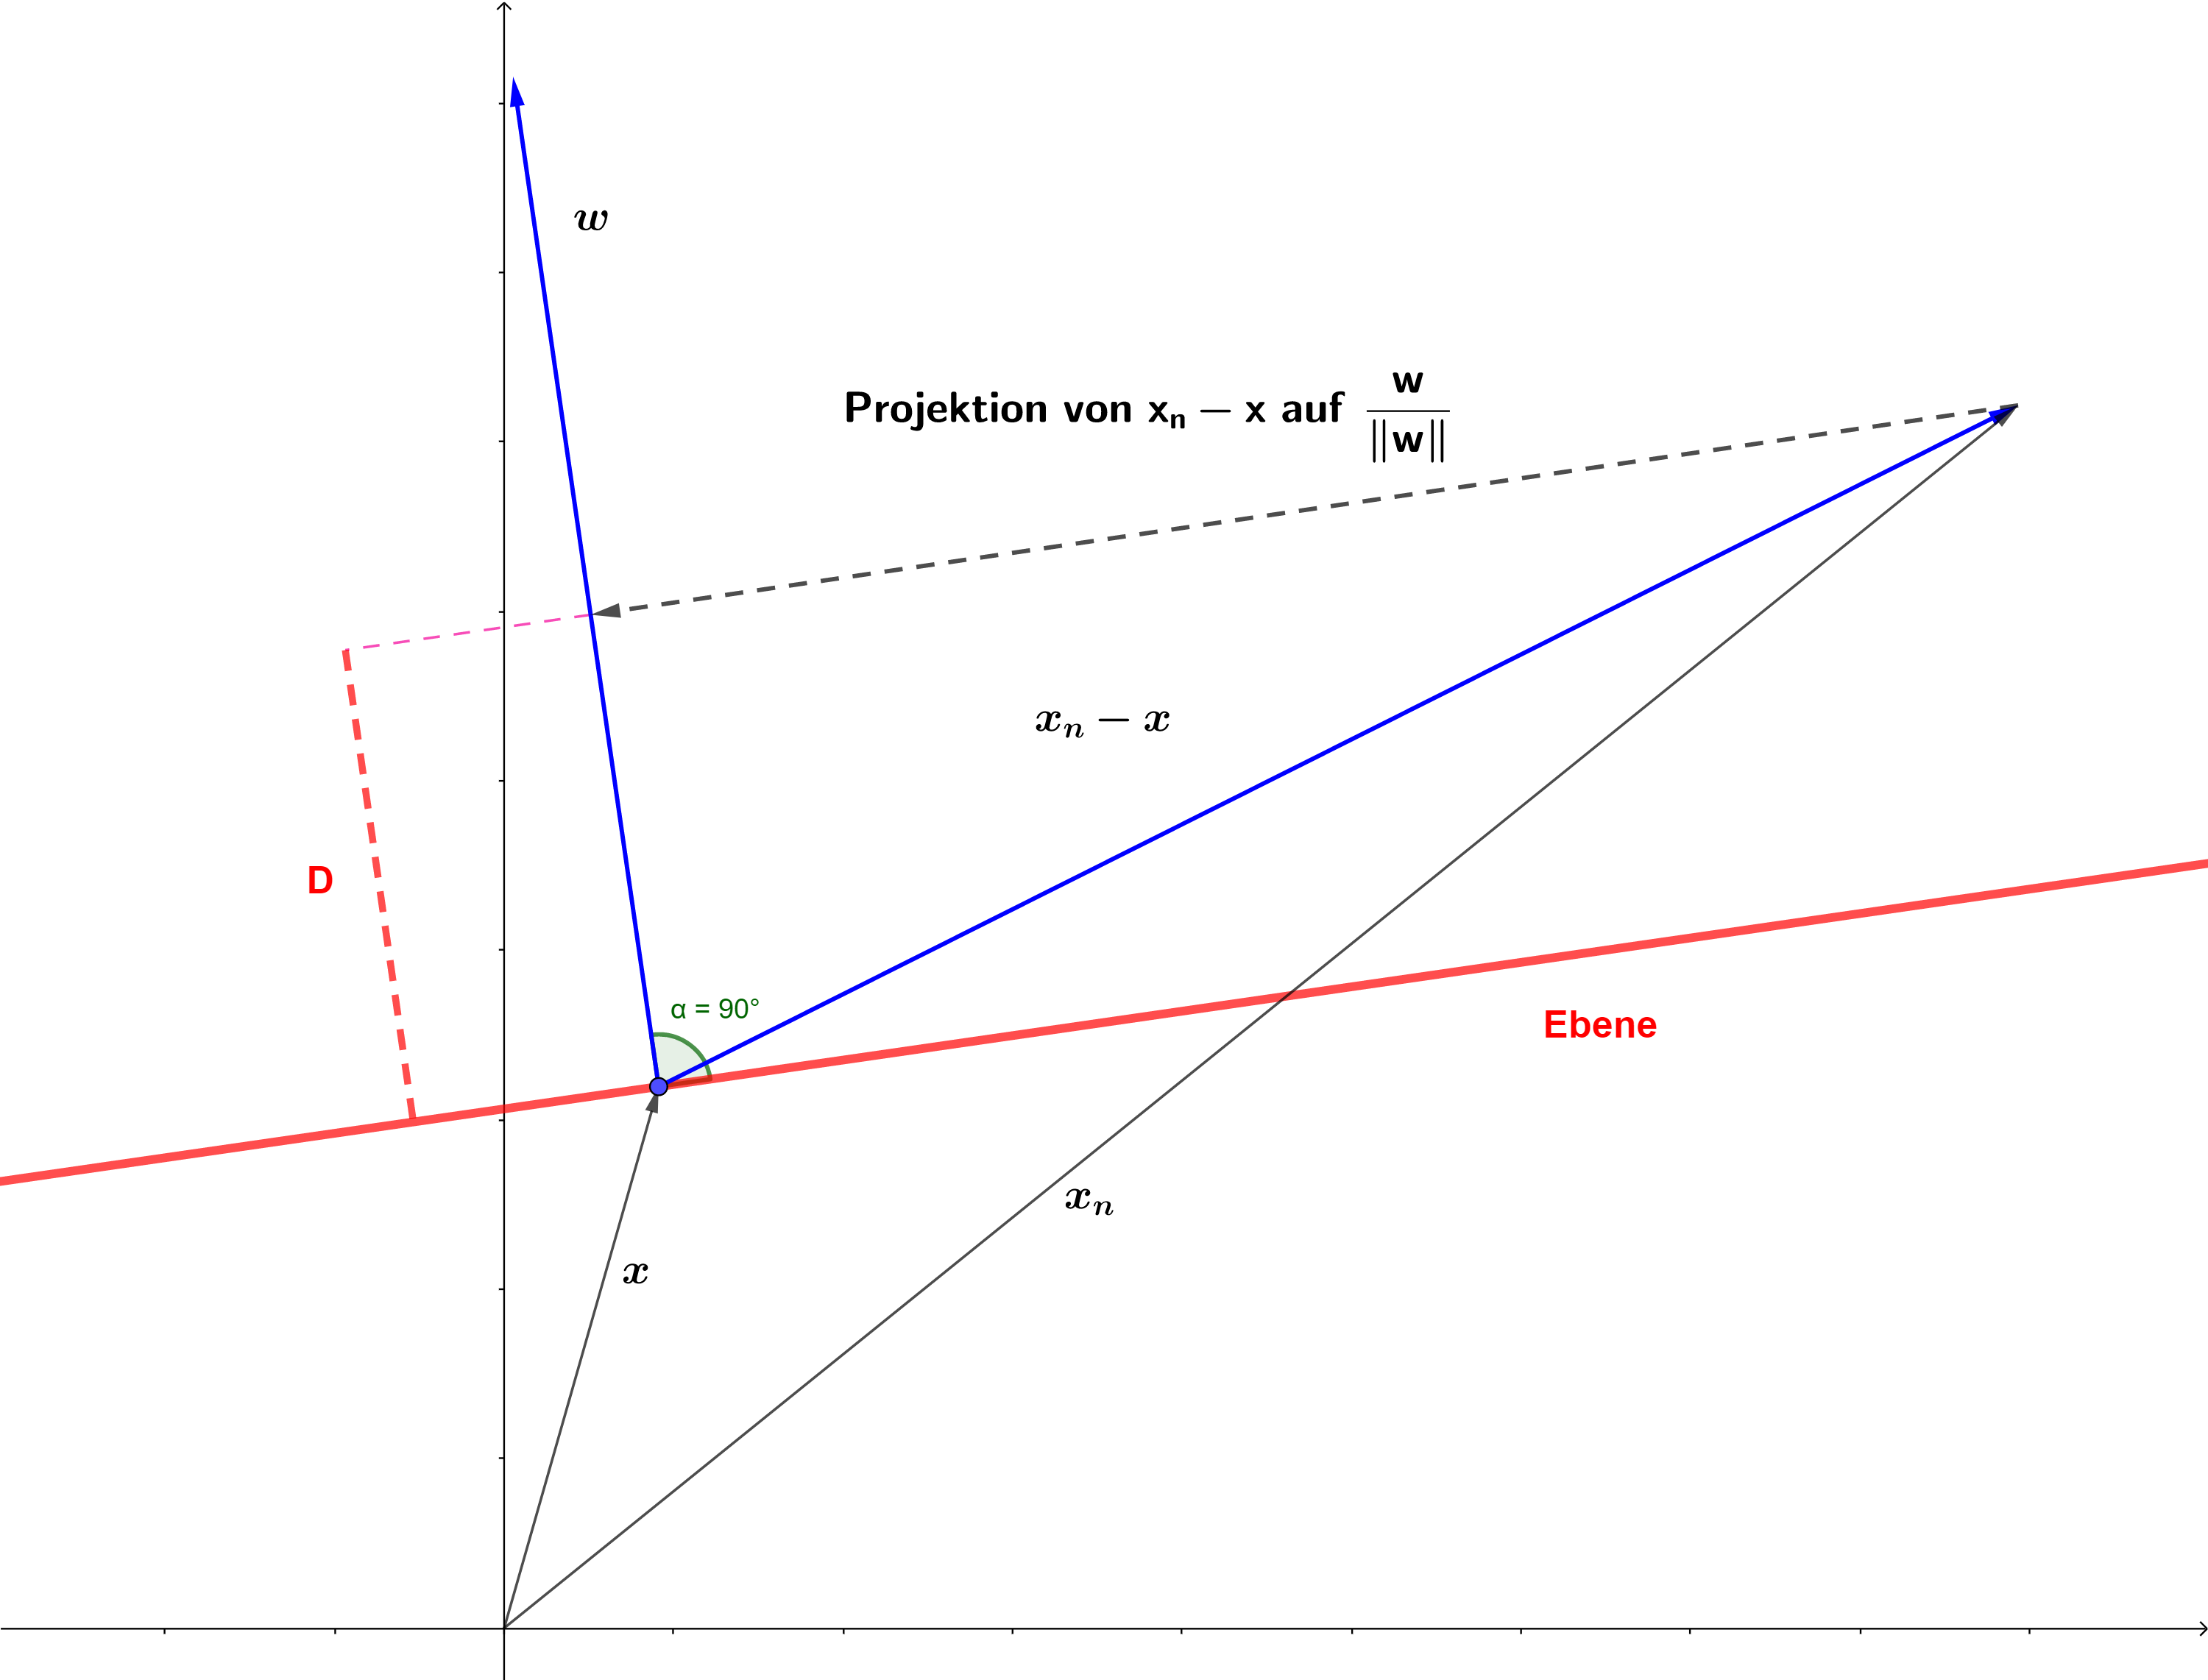
\includegraphics{assets/projection.png}
	\caption{Durch die Projektion von $(x_{k} - x)$ auf den Einheitsvektor von $w$ kann der Normalabstand $D$ von $x_{k}$ zu der Ebene bestimmt werden.}
	\label{fig:projection}
\end{figure}

Weil der Punkt $x$ auf der Ebene liegt gilt $w^{T} x + b = 0$ (\autoref{plane_eq}):
\begin{equation} \label{distance_to_plane_simplified1}
	\begin{aligned}
		D &= \frac{1}{\norm{w}} | (w^{T} x_{k} + b) |
	\end{aligned}
\end{equation}

Aus \autoref{plane_normalization} gilt weiters $| (w^{T} x_{k} + b) | = 1$ wenn $x_{k} = \hat{x}$ der am nächsten zu der Ebene liegende Punkt ist. Somit ergibt sich der kleinste Abstand zur Ebene als:
\begin{equation} \label{distance_to_plane_simplified2}
	\begin{aligned}
		D &= \frac{1}{\norm{w}}
	\end{aligned}
\end{equation}

\subsection{Optimierungsproblem}

\autoref{distance_to_plane_simplified2} beschreibt den Normalabstand zu dem am nächsten an der Ebene liegenden Punkt $\hat{x}$. Ziel einer \ac{SVM} ist die Maximierung dieses Abstands für alle $N$ Eingabevektoren $x_{1}..x_{N} \in \mathbb{R}^{D}$. Hierbei handelt es sich um ein Optimierungsproblem mit Nebenbedingungen:

\begin{subequations}
	\begin{alignat}{2}
		&\!\max_{w}        &\qquad&  \frac{1}{\norm{w}} \label{eq:optProb}\\
		&\text{mit } &      & \min_{n=1..N} |w^{T} x_{n} + b| = 1 \label{eq:constraint1}
	\end{alignat}
\end{subequations}

\autoref{eq:constraint1} beschreibt hier den am nächsten zur Ebene gelegenen Punkt $\hat{x}$ in allgemeiner Form. Der Betrag lässt sich umschreiben durch die Einführung von Labels $y_{n} \in \{-1, +1\}$. Diese beschreiben jeweils die Klasse des zugehörigen Vektors $x_{n}$. Für eine korrekte Klassifizierung der \ac{SVM} gilt:
\begin{equation} \label{svm_classif}
	\begin{aligned}
		y_{n} &= sign(w^{T} x_{n} + b)
	\end{aligned}
\end{equation}

Somit gilt für einen korrekt klassifizierten Vektor $x_{k}$:
\begin{equation} \label{abs_value_trick}
	\begin{aligned}
		|w^{T} x_{n} + b| &= y_{n} (w^{T} x_{n} + b)
	\end{aligned}
\end{equation}


Durch Anwendung von \autoref{abs_value_trick} in \autoref{eq:constraint1}, Umformulierung der zu optimierenden Funktion in eine Minimierung und der Verallgemeinerung von $\hat{x}$ auf beliebige Punkte $x_{n}$ erhält man:
\begin{subequations}
	\begin{alignat}{2}
		&\!\min_{w}        &\qquad&  \frac{1}{2} w^{T} w \label{eq:optProb2}\\
		&\text{mit } &      & y_n (w^{T} x_{n} + b) \geq 1 \text{ für } n=1..N \label{eq:constraint12}
	\end{alignat}
\end{subequations}

Die Verallgemeinerung von \autoref{eq:constraint1} auf \autoref{eq:constraint12} auf beliebige Punkte ist so möglich, weil durch \autoref{plane_normalization} sichergestellt ist, dass der kleinste Wert für $(w^{T} x_{n} + b)$ $1$ ist, und somit die Werte für alle anderen Punkte größer oder gleich $1$ sein müssen. \\

\subsection{Lagrange Optimierung}





% Literaturverzeichnis:
\clearpage
\phantomsection
\addcontentsline{toc}{chapter}{Bibliography}
\printbibliography

\end{document}
